\documentclass{article}
\usepackage[ruled,vlined,linesnumbered]{algorithm2e}
\usepackage{algpseudocode}
\usepackage{amsmath}
\usepackage{amsthm}
\usepackage{graphicx}
\usepackage{subfigure}
\usepackage{float}
\usepackage{amsmath }
\usepackage{amsfonts }
\usepackage{pdfpages}
\usepackage{epsfig}
\usepackage{graphicx}
\usepackage{arydshln}
\usepackage{verbatim}
\usepackage{subfigure}
\usepackage{enumerate}
\usepackage{rotating}
\usepackage{threeparttable}
\usepackage{caption}
\usepackage{epsfig}
\usepackage{cite}
\usepackage{times}
\usepackage{geometry}
\usepackage{tikz}
\geometry{a4paper}
\theoremstyle{definition}
\newtheorem{prob}{Problem}
\newtheorem{ans}{Answer}
\usepackage[colorlinks,linkcolor=black]{hyperref}
\linespread{1.2}
\begin{document}
	\title{AI2702 Mobile Robotics Homework 1}
	\author{Kailing Wang 521030910356}
	\date{March 11.2024}
	\maketitle
	
%	\begin{center}
%		\begin{tikzpicture}
%			
%			% Draw axes
%			\draw[->] (0,0) -- (3,0) node[right] {$X_I$};
%			\draw[->] (0,0) -- (0,3) node[above] {$Y_I$};
%			
%			% Draw the robot body
%			\draw[thick] (1,1) circle [radius=0.02];
%			\draw[thick] (1,1.1) circle [radius=0.05];
%			\draw[thick] (0.5,1) -- (0.5,0.5);
%			\draw[thick] (0.5,1) -- (1.5,1);
%			\draw[thick] (1.5,1) -- (1.5,0.5);
%			\draw[thick] (0.5,0.5) -- (1.5,0.5); % robot body
%			
%			% Draw wheels
%			\draw[thick] (1.5,0.5) circle [radius=0.1];
%			\draw[thick] (0.5,0.5) circle [radius=0.1];
%			
%			% Draw robot local axes
%			\draw[->, dashed] (1,0.5) -- (0,0.5) node[below right] {$Y_R$};
%			\draw[->, dashed] (1,0.5) -- (1,1.5) node[above left] {$X_R$};
%			
%		\end{tikzpicture}
%		
%	\end{center}
	\begin{figure}[ht]
	\centering
	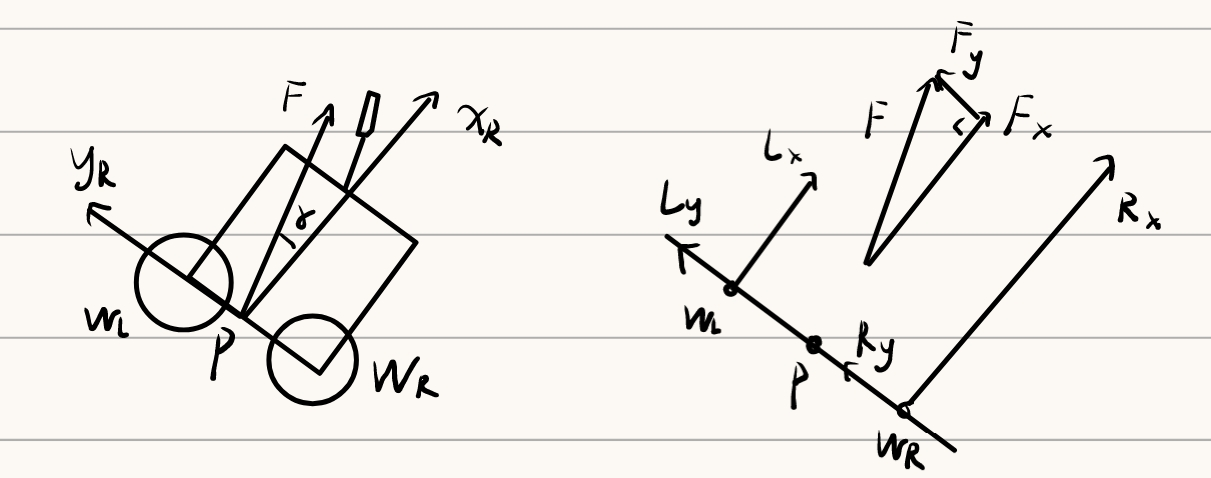
\includegraphics[width=0.8\textwidth]{robot}
	\caption{Robot Structure}
	\label{fig:robot}
	\end{figure}
	Let's start from 
	$$
	\left[\begin{array}{l}
	J_1\left(\beta_s\right) \\
	C_1\left(\beta_s\right)
	\end{array}\right] R(\theta) \dot{\xi}_1=\left[\begin{array}{c}
	J_2 \dot{\varphi} \\
	0
	\end{array}\right].
	$$
	
	However, I find it weird. The constraint seems different than the wheels we know before. At first I tried to model the spherical wheels as parallel steered standard wheels, but I end up with confusion. 
	
	There is a severe problem here. Suppose the robot is moving towards direction $F$ with $\gamma$ from $X_R$. If there is a difference in speed between the wheels that are parallel, the axis of wheels should break. 
	
	Then I consider the case wheels are not parallel. An obvious constraint is that the two wheels always have the same speed on the $Y_R$ direction or the robot explodes. This way, the equations is the same as the case of standard wheels. The coordinate system is defined as in Fig.1. We have $\alpha_L=\frac{\pi}{2}, \beta_L=\beta_1$ for the left wheel and $\alpha_R=-\frac{\pi}{2}, \beta_R=\beta_2$ (yes, index 1 for left and 2 for right):
 	\begin{equation}
	 	\begin{aligned}
	 	r_1\dot\varphi_1\sin \beta_1 &= r_2\dot\varphi_2\sin\left(\beta_2-\pi\right) \\
	 	&= -r_2\dot\varphi_2\sin\beta_2, 
	 	\end{aligned}
 		\label{1}
	 \end{equation}
 	This shows that only $\beta_1$ is a free control variable. 
	
	Then, similar to standard wheels, for spherical wheels:
	\begin{align*}
		[\sin (\alpha+\beta)-\cos (\alpha+\beta)(-l) \cos \beta] R(\theta) \dot{\xi}_1-r \dot{\varphi} &= 0, \\
		[\cos (\alpha+\beta) + \sin (\alpha+\beta) l \sin \beta] R(\theta) \dot{\xi}_1 &= 0,
	\end{align*}
%	here $\alpha_1 = -\frac{\pi}{2}$ for the right wheel and $\alpha_2 = \frac{\pi}{2}$ for the left wheel. $\beta$ is a variable here. Suppose the robot is moving towards a direction that is $\gamma$ with $X_R$. $\beta_1=\pi + \gamma$ and $\beta_2=\gamma$. Further more, we use the same simplification as in the textbook to ignore the castor wheel. That is:

	We use the same simplification as in the textbook to ignore the castor wheel. That is:
	$$
	\left[\begin{array}{ccc}
		\cos\beta_1 & \sin\beta_1 & -l \cos\beta_1 \\
		-\cos\beta_2 & -\sin\beta_2 & -l \cos\beta_2 \\
		-\sin\beta_1 & \cos\beta_1 & l\sin\beta_1 \\
		\sin\beta_2 & -\cos\beta_2 & l\sin\beta_2 \\
	\end{array}\right] R(\theta) \dot{\xi}_1=\left[\begin{array}{c}
		\left[J_2 \dot{\varphi}\right]_{2\times 2} \\
		0 \\
		0
	\end{array}\right].
	$$
	
	Simplify the above system of equations by using linear combinations of the first three rows with coefficients $[\sin\beta_1, \sin\beta_2, \cos\beta_1]$ to obtain:
	\begin{equation}
		\left[-\sin\beta_2\cos\beta_2, 1-\sin^2\beta_2, -l\sin\beta_2\cos\beta_2\right]R(\theta) \dot{\xi}_1=[r_1\dot\varphi_1\sin \beta_1 + r_2\dot\varphi_1\sin \beta_2], 
	\end{equation}
	and if we substitute equation \ref{1}, we get the fourth row. Thus we prove the fourth equation do not add more constraint. In fact, we'd arbitrarily choose the third or the fourth row to calculate inv.
	
	The result is:
	\begin{align}
		\dot{\xi}_I=R(\theta)^{-1}\left[\begin{matrix}- \frac{\sin{\left(\beta_{1} \right)} \tan{\left(\beta_{2} \right)}}{2} + \frac{\cos{\left(\beta_{1} \right)}}{2} & - \frac{1}{2 \cos{\left(\beta_{2} \right)}} & - \frac{\sin{\left(\beta_{1} + \beta_{2} \right)}}{2 \cos{\left(\beta_{2} \right)}}\\ \sin{\left(\beta_{1} \right)} & 0 & \cos{\left(\beta_{1} \right)}\\ - \frac{\sin{\left(\beta_{1} \right)} \tan{\left(\beta_{2} \right)} + \cos{\left(\beta_{1} \right)}}{2 l} & - \frac{1}{2 l \cos{\left(\beta_{2} \right)}} & \frac{\sin{\left(\beta_{1} - \beta_{2} \right)}}{2 l \cos{\left(\beta_{2} \right)}}\end{matrix}\right]\left[\begin{array}{c}
			\left[J_2 \dot{\varphi}\right]_{2\times 2} \\
			0
		\end{array}\right],
	\end{align}
	Note that since $\beta_2$ can be presented with other control variables in equation \ref{1}, this expression has many equivalent forms. Also the definition of $\beta_1$ and $\beta_2$ would cause the result to differ. 
	
	If we use the fourth row, the result is:
	\begin{align}
		\dot{\xi}_I=R(\theta)^{-1}\left[\begin{matrix}
			\frac{1}{2 \cos{\left(\beta_{1} \right)}} & - \frac{\cos{\left(\beta_{1} + \beta_{2} \right)}}{2 \cos{\left(\beta_{1} \right)}} & \frac{\sin{\left(\beta_{1} + \beta_{2} \right)}}{2 \cos{\left(\beta_{1} \right)}}\\
			0 & - \sin{\left(\beta_{2} \right)} & - \cos{\left(\beta_{2} \right)}\\
			- \frac{1}{2 l \cos{\left(\beta_{1} \right)}} & - \frac{\cos{\left(\beta_{1} - \beta_{2} \right)}}{2 l \cos{\left(\beta_{1} \right)}} & - \frac{\sin{\left(\beta_{1} - \beta_{2} \right)}}{2 l \cos{\left(\beta_{1} \right)}}
		\end{matrix}\right]\left[\begin{array}{c}
			\left[J_2 \dot{\varphi}\right]_{2\times 2} \\
			0
		\end{array}\right],
	\end{align}
	
	The matrix inv above is calculated and converted to latex with sympy.
	
	
%	$$
%	\left[\begin{array}{ccc}
%		\cos\gamma & \sin\gamma & l \cos\gamma \\
%		\cos\gamma & \sin\gamma & -l \cos\gamma \\
%		-\sin\gamma & \cos\gamma & -l\sin\gamma \\
%		-\sin\gamma & \cos\gamma & l\sin\gamma \\
%	\end{array}\right] R(\theta) \dot{\xi}_1=\left[\begin{array}{c}
%		J_2 \dot{\varphi} \\
%		0
%	\end{array}\right].
%	$$
%	Similarly, the two wheels always have parallel
	
%	\begin{equation*}
%		\dot{\xi}_I=R(\theta)^{-1}\left[\begin{array}{ccc}
%			1 & 0 & 1 \\
%			1 & 0 & -1 \\
%			0 & 1 & 0
%		\end{array}\right]^{-1}\left[\begin{array}{c}
%			J_2 \varphi \\
%			0
%		\end{array}\right]=R(\theta)^{-1}\left[\begin{array}{ccc}
%			\frac{1}{2} & \frac{1}{2} & 0 \\
%			0 & 0 & 1 \\
%			\frac{1}{21} & -\frac{1}{21} & 0
%		\end{array}\right]\left[\begin{array}{c}
%			J_2 \varphi \\
%			0
%		\end{array}\right] 
%	\end{equation*}	
%	\begin{equation*}
%		\dot{\xi}_I=R(\theta)^{-1}\left[\begin{array}{ccc}
%			\frac{1}{\sqrt{3}} & 0 & -\frac{1}{\sqrt{3}} \\
%			-\frac{1}{3} & \frac{2}{3} & -\frac{1}{3} \\
%			-\frac{1}{31} & -\frac{1}{31} & -\frac{1}{31}
%		\end{array}\right] J_2 \dot{\varphi}
%	\end{equation*}	
%	
%	\begin{equation*}
%		\dot{\xi}_I = R(\theta)^{-1} \left[\begin{array}{ccc}
%			\frac{1}{2} & \frac{1}{2} & 0 \\
%			0 & 0 & 1 \\
%			\frac{1}{2L} & -\frac{1}{2L} & 0
%		\end{array}\right] \left[\begin{array}{c}
%			J_2 \varphi \\
%			0
%		\end{array}\right]
%	\end{equation*}
%	\begin{equation*}
%		\dot{\xi}_I = R(\theta)^{-1} \left[\begin{array}{ccc}
%			\frac{1}{\sqrt{3}} & 0 & -\frac{1}{\sqrt{3}} \\
%			-\frac{1}{3} & \frac{2}{3} & -\frac{1}{3} \\
%			-\frac{1}{3L} & -\frac{1}{3L} & -\frac{1}{3L}
%		\end{array}\right] J_2 \dot{\varphi}
%	\end{equation*}
	
\end{document}
